\chapter{Oprogramowanie symulacyjne}
\label{ch:simulation-app}

Na potrzeby pracy zostało stworzone oprogramowanie symulacyjne, które posłużyło do przeprowadzenia testów algorytmów planowania tras oraz wizualizacji ich działania.
W tym rozdziale opisano techniczne rozwiązania wykorzystane podczas tworzenia oprogramowania.
W aplikacji zostały zaimplementowane algorytmy planowania tras opisane w rozdziale \ref{ch:alg-impl}.
Prezentacja ich działania odbywa się poprzez wizualizację ruchu robotów mobilnych w czasie rzeczywistym. 

\section{Funkcjonalności aplikacji}
Aplikacja umożliwia dowolne definiowanie przez użytkownika środowiska, w którym poruszają się roboty. Obejmuje to:
\begin{itemize}
	\item wybór rozmiaru mapy - dowolną wysokość oraz szerokość. Mapa nie musi być kwadratowa.
	\item możliwość wygenerowania mapy za pomocą generatora labiryntów (por. \ref{ch:mazegen}) lub manualnego umieszczania przeszkód na mapie za pomocą myszki,
	\item wybór liczby robotów i dokonanie ich automatycznego rozmieszczenia na mapie (w losowych polach z pominięciem pól zajętych). Użytkownik ma także możliwość manualnego dodawania i usuwania robotów.
\end{itemize}

Aplikacja przeprowadza symulację ruchu robotów w czasie rzeczywistym. W oprogramowaniu zostały zaimplementowane trzy algorytmy planowania ruchu robotów. Są to:
\begin{itemize}
	\item Metoda pól potencjałowych (por. \ref{ch:potential-fields})
	\item Local-Repair A* (por. \ref{ch:alg-collision-avoid})
	\item Windowed Hierarchical Cooperative A* (por. \ref{ch:alg-whca})
\end{itemize}
Wizualizacja każdego z tych algorytmów dostępna jest na osobnej zakładce w aplikacji.

\section{Graficzny interfejs użytkownika}
Graficzny interfejs użytkownika stanowi desktopowa aplikacja okienkowa, której głównym elementem jest panel zakładek. Każda z zakładek reprezentuje wizualizację osobnego algorytmu planowania ruchu robotów.

Z myślą o spopularyzowaniu opracowanych algorytmów, elementy interfejsu użytkownika (takie, jak etykiety lub przyciski) posiadają tekst w języku angielskim.

Pod każdą z zakładek aplikacji układ wizualny jest podobny. Poniżej opisano graficzny interfejs użytkownika wspólny dla wszystkich zakładek.

Po prawej stronie znajduje się panel przycisków akcji oraz panel rozwijanych właściwości z konfiguracją parametrów mapy oraz symulacji. Natomiast po lewej stronie wyświetlany jest obecny stan mapy i położenia robotów mobilnych. Mapa wyświetlana jest z zaznaczeniem linii siatki pól obrazujących liczbę pól na mapie. Przeszkody wyświetlane są jako czarne kwadraty, zaś roboty jako kolorowe wypełnione koła.
Kliknięcie prawym przyciskiem myszy (również z możliwością ciągłęgo przytrzymania) powoduje wstawienie lub usunięcie przeszkody na mapie w odpowiednich polach.
Punkty docelowe, do których podążąją roboty wyświetlane są jako krzyżyki w kolorze takim samym, jaki został przypisany do robota. Liczba robotów nie jest ograniczona przez aplikację. Aby odróżniać roboty między sobą, każdy robot otrzymuje inny kolor wynikającą z równego podziału palety HSV według barwy (ang. {\it hue}) na liczbę robotów.

Okno aplikacji jest skalowalne i w pełni responsywne. Po zmianie rozmiaru okna przez użytkownika rozmiar mapy dopasowuje się do maksymalnego obszaru, jaki może zająć (z zachowaniem proporcji wymiarów mapy).

Symulacja ruchu robotów rozpoczyna się jak tylko zostanie wyznaczony punkt docelowy dla robota. Dzięki temu, że wykonywanie obliczeń planowania tras zostało przeniesione do osobnych wątków, uzyskano płynność animacji ruchu robotów mobilnych. Uniknięto również problemu braku odpowiedzi interfejsu użytkownika podczas planowania trajektorii.

\subsection{Metoda pól potencjałowych}
Na pierwszej zakładce "Potential fields" w oknie aplikacji przedstawiona jest wizualizacja metody pól potencjałowych.

\begin{figure}
	\centering
	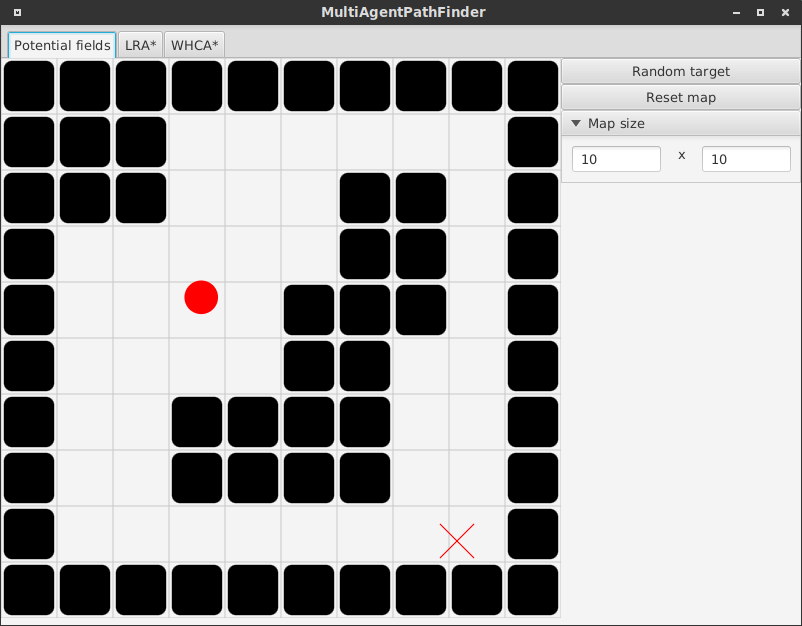
\includegraphics[width=0.8\columnwidth]{img/robopath/ui-fields}
	\caption{Zrzut ekranu aplikacji w trakcie wizualizacji metody pól potencjałowych.}
	\label{fig:robopath-ui-fields}
\end{figure}

Na panelu konfiguracji parametrów, użytkownik może wybrać dowolny rozmiar mapy, podając szerokość i wysokość wyrażone w liczbie pól.
Po naciśnięciu przycisku "Reset map" tworzona jest nowa mapa o zadanych rozmiarach, natomiast pozycja początkowa robota zostaje wylosowana.
Naciśnięcie przycisku "Random target" powoduje wyznaczenie losowego punktu na mapie jako cel dla robota i rozpoczęcie podążąnia za nim.

Klikając lewym przyciskiem myszy na mapie, Użytkownik może manualnie wskazać punkt docelowy dla robota.
Planowanie i symulacja ruchu robota odbywa się w trybie ciągłym. Robot nie jest ograniczony zdyskretyzowaną siatką pól na mapie, jego przestrzeń poruszania się jest ciągła.

\subsection{Local-Repair A*}
\label{ch:app-lra}
Pod kolejną zakładką "LRA*" w oknie aplikacji dostępna jest wizualizacja metody algorytmu bazującego na A* z lokalną detekcją i rozwiązywaniem kolizji.

Na panelu konfiguracji parametrów w sekcji "Map size", użytkownik może wybrać dowolny rozmiar mapy, podając szerokość i wysokość wyrażone w liczbie pól.
Po naciśnięciu przycisku "Reset map" tworzona jest nowa, pusta mapa o zadanych rozmiarach.
W sekcji "Robots" użytkownik wybiera liczbę robotów (do automatycznego rozmieszczenia) oraz ma możliwosć zaznaczenia opcji "auto-assign next target", co skutkuje automatycznym wyznaczaniem kolejnego punktu docelowego, dla robota, który dotarł do poprzedniego celu.
Przycisk "Generate maze" pozwala na wygenerowanie labiryntu przy użyciu generatora map (por. \ref{ch:mazegen}).
Przycisk "Place robots" usuwa wszystkie roboty z mapy i umieszcza na niej wybraną przez użytkownika liczbę robotów w losowych miejscach na mapie (za wyjątkiem zajętych przez przeszkody oraz inne roboty).
Przycisk "Random target" losuje punkty docelowe dla wszystkich robotów. Każdy z agentów otrzymuje inny punkt docelowy (nie będący przeszkodą), do którego zmierza. Nadanie punktów docelowych powoduje rozpoczęcie planowania trajektorii i symulację ruchu agentów.

Klikając lewym przyciskiem myszy na mapie, Użytkownik może utworzyć nowego robota. Nowemu agentowi zostaje przydzielony punkt docelowy w miejscu, w którym lewy przycisk myszy został zwolniony.
Dodatkowo pokazywane są zaplanowane ścieżki dla każdego robota. Wyświetlane są jako linie łamane w kolorze takim samym, jaki odpowiada robotowi.
Nad robotem, w jego aktualnym położeniu wyświetlany jest jego numer (identyfikator).

\begin{figure}
	\centering
	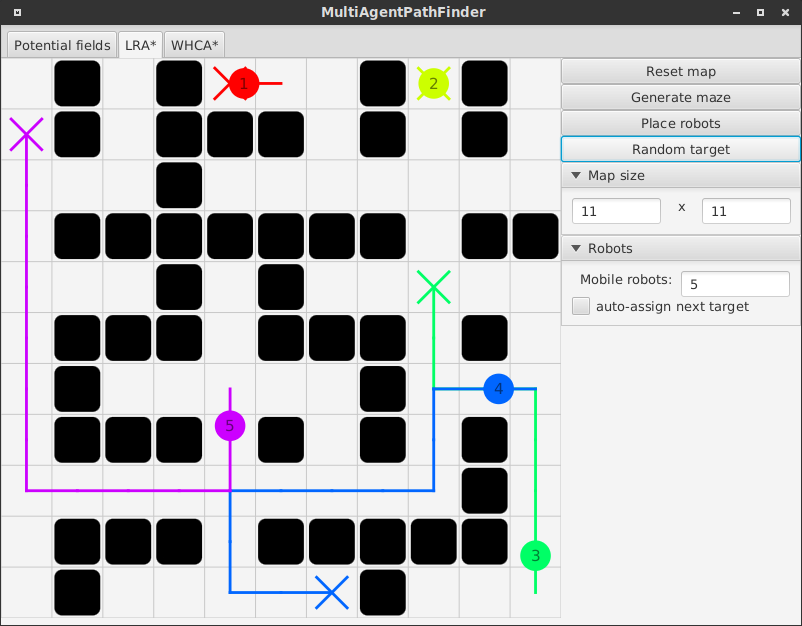
\includegraphics[width=0.8\columnwidth]{img/robopath/ui-lra}
	\caption{Zrzut ekranu aplikacji w trakcie wizualizacji metody Local-Repair A*.}
	\label{fig:robopath-ui-lra}
\end{figure}


\subsection{Windowed Hierarchical Cooperative A*}
Pod ostatnią zakładką "WHCA*" w oknie aplikacji dostępna jest wizualizacja metody kooperacyjnego planowania tras dla wielu robotów z planowaniem odbywającym się w ograniczonym oknie czasowym.

Interfejs użytkownika jest praktycznie taki sam, jak w przypadku opisanej metody LRA* (por. \ref{ch:app-lra}).
Różni się obecnością dodatkowej sekcji "WHCA*" na panelu konfiguracji z polem "Time window", które pozwala na zmianę wielkości okna czasowego dla algorytmu WHCA*. W wyniku dynamicznego przydzielania priorytetów wielkość ta może zostać zwiększana automatycznie podczas symulacji.
Dodatkowy przycisk "Restore positions" pozwala na cofnięcie stanu robotów do momentu, tuż przed rozpoczęciem symulacji (zaraz po przydzieleniu punktów docelowych). Pozwala to na ponowną obserwację przebiegu symulacji dzięki przywróceniu położenia i stanu agentów.

Nad robotem, w jego aktualnym położeniu wyświetlany jest jego numer (identyfikator) oraz priorytet (oddzielony kropką). Priorytet może być zmienny w trakcie symulacji (w przeciwieństwie do identyfikatora). Początkowo robot zawsze ma priorytet równy identyfikatorowi. Większa wartość priorytetu względem pozostałych oznacza pierwszeństwo uwzględniane podczas planowania tras.

\begin{figure}
	\centering
	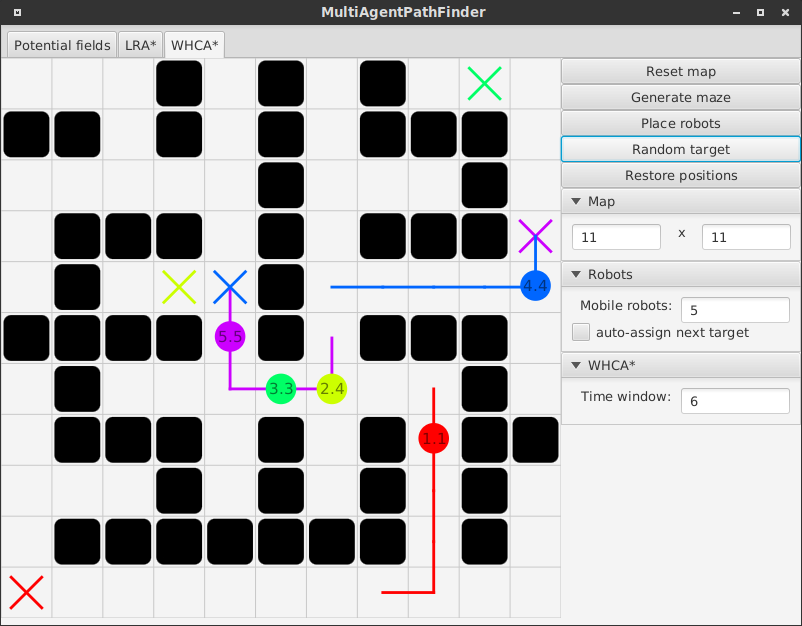
\includegraphics[width=0.8\columnwidth]{img/robopath/ui-whca}
	\caption{Zrzut ekranu aplikacji w trakcie wizualizacji metody Windowed Hierarchical Cooperative A*.}
	\label{fig:robopath-ui-whca}
\end{figure}


\section{Wykorzystane technologie}
$TODO$ stack technologiczny, Wykorzystane technologie i narzędzia - opis technologii:
Java 8 - lambda, functional interfaces, streamy,
Java FX - FXML, Spring (core): IoC, DI; Spring Boot, testy jednostkowe jUnit, git, IntelliJ Ultimate, Maven, Linux, logback, Guava - joiner

uruchomienie aplikacji z kodów źródłowych : mvn spring-boot:run

\section{Testy}
$TODO$ TDD - Test driven development, testy jednostkowe do algorytmów pathfinding

\section{Struktura aplikacji}
$TODO$ lista beanów / serwisów, struktura widok, prezenter, kontroler; osobny wątek w tle do obliczeń + synchronizacja, wątek UI - zapewnienie REal-time, prawie MVP


\section{Screeny}
$TODO$ screeny

\section{Zaimplementowane metody}
$TODO$ potential fields, A*, LRA*, WHCA*

\section{featurey}
ustawianie random seeda
ponowne wykonanie symulacji - te same warunki
przełaczanie między metodami na zakładkach ?
wykonanie symulacji w pojedynczych krokach
resizable window - responsive
heuristic cache
działania na wektorach, immutable vector

\section{Ograniczenia}
$TODO$ nałożone uproszczenia: ruch skośny trwa tyle samo, czas dyskretny, brak czasu na obrót

$TODO$ publikacja na GitHub, licencja MIT, filmiki na YT